% !TEX root = ../main.tex

%% 分析与讨论	
%\begin{table}
%	\renewcommand\arraystretch{1.7}
%	\begin{tabularx}{\textwidth}{|X|X|X|X|}
%		\hline
%		Major：& Physics &Grade：& 2022\\
%		\hline
%		Name： & 杨舒云 \& 戴鹏辉 & Student number：& 22344020 \& 22344016\\
%		\hline
%		Date：& 2024/10/25 & Score： &\\
%		\hline
%	\end{tabularx}
%\end{table}
\section{APL1-1-A 电阻热噪声及玻尔兹曼常量测量 \\ Analysis \& Discussion}


%---------------------------------------------------------------------
% 数据处理
\subsection{Data Processing}

% 分析
\subsubsection{Analysis}
本小节展示实验方案预期的\textbf{数据分析}。
\begin{enumerate}
	\item 数据质量评定
	
	按照讲义要求，为了说明所采数据X或Y是随机噪声和X的采样是独立的，我们可以对采集到的数据进行如下分析：X-Y数据相关性、X或Y数据自相关性，正则分布，简化卡方值。
	
	事实上，在\cite{c}中已经提供了很好的范例，我们可以仿照其1.2.2小节进行，预期得到类似于图2和表1的结果。计划实验前或者过程中，小组中一人预编写处理数据的相关Python脚本。
	
	\item 计算噪声强度
	
	预计采用两种方案：
	\begin{enumerate}
		\item 直接采样计算，按\textbf{原理概述（Principle）}中所讲的，利用时域上的采样计算方均根。
		\item 手动计算：按\textbf{原理概述}部分建议，手动多次记录X、Y值并计算方均根。
	\end{enumerate}
	
	\item 电阻热噪声测量值的输入带宽修正、扣除本底
	
	直接利用\textbf{原理概述}中的理论，进行修正。但是需要考虑的是得想清楚各修正参数如何取值，这个问题搞不明白建议到时候直接咨询老师。此外，还要注意对每组参数对应本底噪声的测量。
	
	\item 噪声获得热噪声、 噪声功率谱密度计算、 玻尔兹曼常量计算
	
	按\textbf{原理概述}部分给出的想法，最基础的是用各组数据测量出的结果分别计算，后续考虑求均值等进一步处理。理想中考虑做随温度变化的噪声测量，利用拟合的方法来获得玻尔兹曼常量结果。
	
	\item 误差分析
	
	这里参考\cite{g}和\cite{c}中内容提出误差分析的方案。
	
	首先根据\cite{g}，假设\textbf{锁相放大器的数值低通滤波器的相对误差可以忽略不计}，电阻 $R$，温度 $T$ 独立测量，其\textbf{误差主要取决于测量仪器的系统误差}。由误差传递可得 $k_B$ 的比值不确定度为：
	\[
	\frac{\delta k_B}{k_B} = \frac{1}{4} \left(\sqrt{\left( 1 + 2 \frac{n_{Bx}^2}{n_{Tx}^2} \right) \frac{8}{M - 1} + \frac{\delta R}{R} + \frac{\delta T}{T}}\right)
	\]
	
	接下来，\cite{c}对上述误差作了进一步讨论，它采用了基于\cite{g}的“保守估计”，取热噪声测量 3 倍标准差 $3\sigma_{n_{TX}}$ (置信度 99.7\%) 计算玻尔兹曼常量测量的最大不确定度为：
	\[
	\frac{\delta k_B}{k_B} = 3\sqrt{\left(1 + 2\frac{n_{BX}^2}{n_{TX}^2}\right)\frac{2}{M-1} + \left|\frac{\delta R}{R}\right| + \left|\frac{\delta T}{T}\right| + 2\frac{\delta \alpha}{\alpha}} \cdot
	\tag{6}
	\]
	其中，电阻与温度的测量随机误差远小于 1\%，可忽略。
	这里只考虑系统误差：设手持多用表测量电阻最大不确定度 $\delta R = 1 \, \Omega$，测温仪在室温和液氮下测温最大不确定度 $\delta T$ 为 0.3 K 和 2 K；
	OE1022 手册中给出的 $\delta \alpha/\alpha \leq 1\%$，标准为 2\%。
	
	此外，它还提到了输入带宽修正也会给测量电压带来比值不确定度 $\delta v_{\text{BW}} / v_{\text{BW}}$，具体表示为
	\[
	\frac{\delta v_{\text{BW}}}{v_{\text{BW}}} = 
	\left( 1 + \frac{n_{BX}^2}{n_{TX}^2} \right)
	\frac{ \left( \omega R_{\text{in}} C_{\text{in}} \right)^2 }{ 1 + \left( \omega R_{\text{in}} C_{\text{in}} \right)^2 }
	\left( \frac{\delta R_{\text{in}}}{R_{\text{in}}} + \frac{\delta C_{\text{in}}}{C_{\text{in}}} \right).
	\]
	
	最后，两篇文献中都提到了现场测量的误差比遥测更大，例如\cref{fig:apl11aenvnoise}所示。
	
	\begin{figure}[h!]
		\centering
		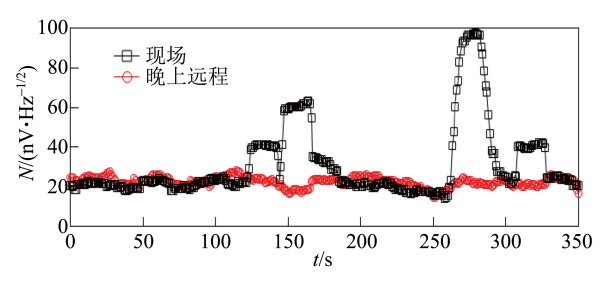
\includegraphics[width=0.5\linewidth]{images/APL1_1_A_env_noise}
		\caption{环境噪声的影响（来自\cite{c}）}
		\label{fig:apl11aenvnoise}
	\end{figure}。
	
	事实上，我们考虑一方面还需查找更多资料做更完善更全面的误差分析；另一方面我们需要结合实验结果进行具体的误差分析。
	
\end{enumerate}

% 讨论
\subsubsection{Discussion}
本小节展示实验方案预期的\textbf{实验结果讨论}。
\begin{enumerate}
	\item 对 A-B 差分输入做输入带宽修正， 其等效输入电阻、 电容怎么取？
	
	\item 经输入带宽修正后的噪声谱密度是否符合热噪声的频谱特征（与频率无关） ？
	
	\item 共用X和Y数据处理得到的$k_B$值求平均是否可以降低其随机误差？
	
	\item 能否通过噪声谱密度计算不同频率下的$k_B$值及其算术平均值$\bar{k_B}$？
	
	\item 本底噪声与仪器和测量时段有关， 输入带宽修正因子与电缆温度有关（参考\cite{c}）。
\end{enumerate}

%% 总结
%\subsubsection{Conclusion}
%\begin{itemize}
%	\item 
%\end{itemize}


%---------------------------------------------------------------------
% 实验后思考题
\subsection{Reflections after Experiment}
实验过程中需注意对以下问题做考虑：

%思考题1
\begin{question}
	样品盒及传输电缆是否会对本底有贡献？ 用实验现象回答： 处于不同环境（如人的触碰、或插入液氮瓶后） 是否对测量产生影响？
\end{question}

% 思考题2
\begin{question}
	采样时间间隔$\Delta t$约多少个时间常数时，X任意相邻采样读数$X(t)$与$X(t+\Delta t)$可视独立无关的？如何验证？如想缩短测量时间并要求采样读数保持随机噪声特性，选择时间常数为多长合适？
\end{question}

\subsection{Statement}
\begin{itemize}
	\item 尽管前面提到这篇实验方案中不考虑远程测量（所谓“遥测”），但是再进一步的资料查找阅读中，从\cite{c}和\cite{g}中了解到环境噪声的影响是比较大的：
	
	“近代物理教学实验室的空调和风机每天24小时不间断运行，但学生没有测量环境噪声频谱，因而尚不能排除实验时他们取选的参考频率与环境噪声频率相近的可能性”；
	
	“在教学实验对电磁干扰屏蔽能力有限的条件下，为减少环境噪声的影响，可将实验安排在下班后，采取远程测量方式进行，要求实验现场无人，且除电脑和锁相放大器外的其他电器设备关闭.在本教学实验室的实验表明，环境噪声的影响能下降到热噪声或更低的水平”。
	
	因此，我们的计划是这样的：先按实验方案完成现场的测量，在此基础上我们在现场进一步考虑遥测的方案，并考虑与当天晚上进行测量（但是我们对实验进度的推荐持悲观的态度，很担心我们或者其它同学晚上仍在进行实验，这样是不会减少环境噪声的），预计第二天早上对数据进行验收。
	
	\item \textbf{\textcolor{fred}{这一点对老师已经提出的提出的修改意见做回应：}}
	\begin{enumerate}
		\item 用$\Delta\nu$标记频率的记法是按\cite{a}给出的，本实验方案中已修改。
		
		\item 关于电阻随温度会变化的问题，目前已将方案改为：
		
		基于$k_B = \dfrac{v_{Nx}^2}{4\times\text{ENBW}\times TR}$，我们可以考虑一种变温测量下的\textbf{线性拟合方案}，即用变化的温度与阻值（阻值也会随温度变化）乘积作为梯度测量下的功率谱变化的斜率以表征玻尔兹曼常数：
		$$
		\dfrac{v_{Nx}^2}{\text{ENBW}}=4k_B\times TR
		$$
		
		\item 关于频率点的分配，实际上我们对此没有什么头绪。我们的想法是：按\cref{fig:effect-of-bandwidth-on-selecting-noise}，噪声在频域上是均匀分布的，因此每组同学只要多选几个频率点进行测量，也许不太需要考虑频率覆盖的问题（真不太确定）？
		
		\item 关于使用AI工具的问题：在我们看来，\textbf{AI工具和搜索引擎差不多}，或者说它就是一种用于更迅速的查找资料的搜索引擎。如果老师用AI工具较多的话，应该会注意到AI的回答有着如图所示明显的“分点作答”的风格：
		
		\begin{figure}[h!]
			\centering
			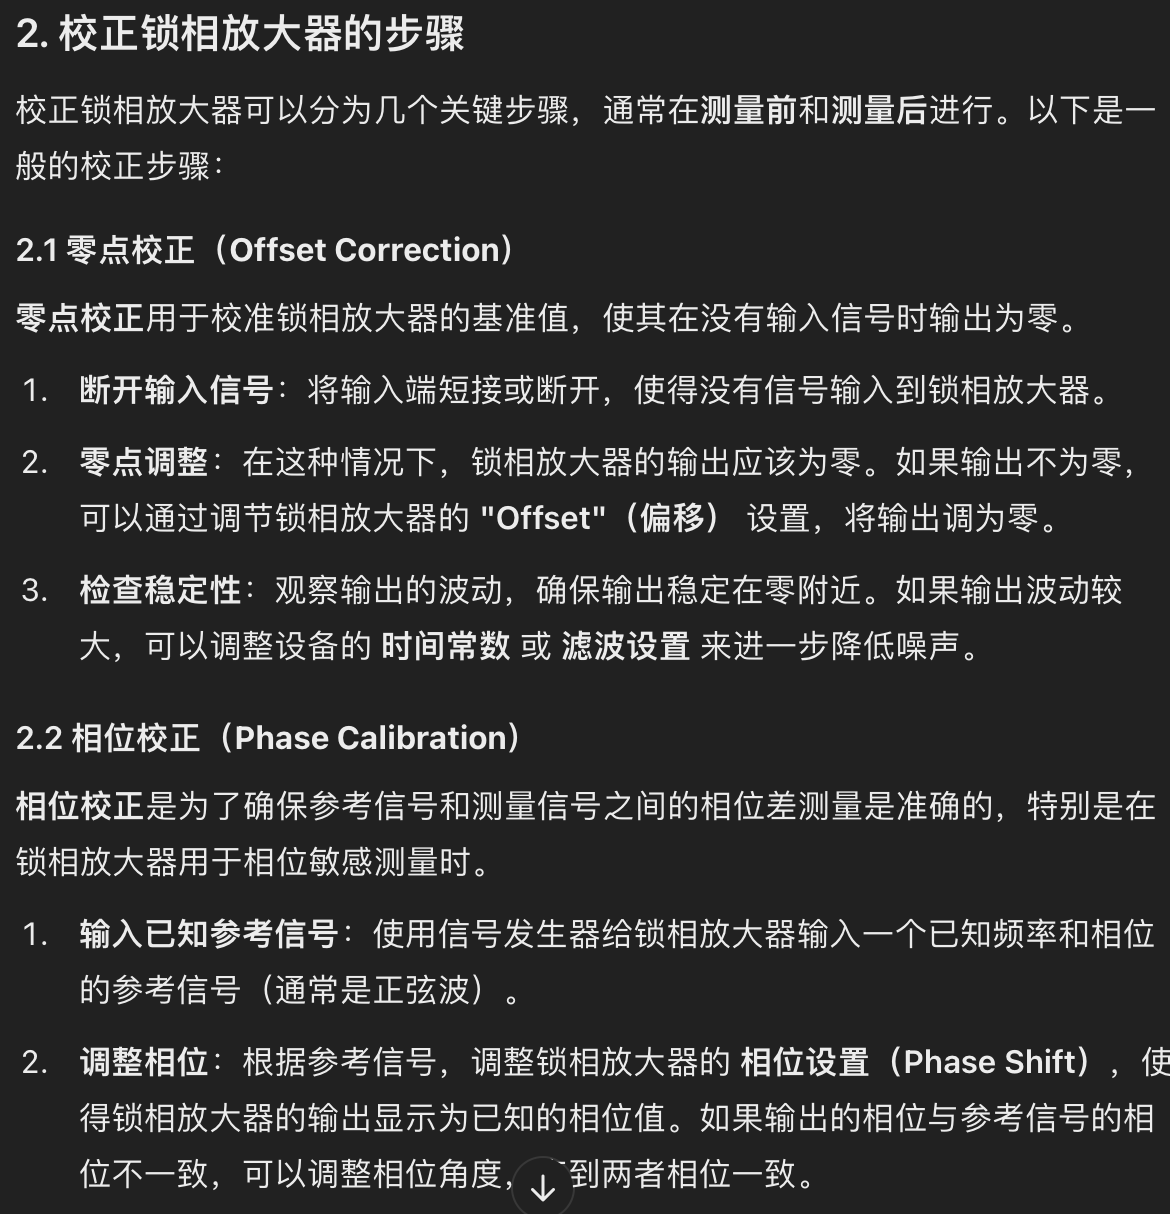
\includegraphics[width=0.5\linewidth]{images/APL1_1_A_AI}
			\caption{AI回答与个人回答是不同的}
			\label{fig:apl11aai}
		\end{figure}
		
		而我们的回答正是相当于“利用搜索引擎查找资料后整理得到的”（这一点从这篇方案中涉及到的参考文献的数目也可以看出，我们的确是去查找了不少资料的）。
		
		其中，关于频率分配的问题的回答我们最根本的想法如上所示，关于这一点我们讨论后决定在现场听老师是否有更完善更合理的解释和安排，因此回答内容主要是由AI给出的一个“也许会有启发性的方案”。
		
		关于校正的问题，首先老师应当注意到了我们基于这个回答在步骤中考虑并引入了校正的过程（主要是零点校正和本底输入带宽校正），其中由于本底输入带宽校正在原理概述中详细讨论了，所以回答中比较简略。
		
		关于环境噪声的问题，最初在完成这个问题时，我们确实对此没什么概念，对环境噪声的较深刻的印象来自于我们阅读\cite{c}和\cite{g}后。我们的基本的考虑是环境噪声会明显导致噪声的频域分布不再均匀（如1/f噪声、市电50Hz），正如我们在回答中所写。此外，正如我们在上面谈到的那样，减小环境噪声较为有效的方案还是遥测。
		
		\item “10ms行不行？”关于这个问题，我们在写这篇方案的时候实际上有简单的思考：首先时间常数决定了滤波器的带宽，时间常数太小时（如10ms时），带宽太大，可能会引入1/f这样的环境噪声，这在实验步骤的描述中提到了：“由于测量装置不可能完全屏蔽环境干扰，选择太大的带宽容易引入近频的环境噪声”。此外，参考\cite{c}和\cite{g}，它们举例时考虑的时间常数都比较大。而我们在前一次实验中也有经验，时间常数大一些时信号会更稳定。因此，我们保守的认为10ms不太行，要选大一点的时间常数。
	\end{enumerate}
	
	\item 上述实验方案有很多不足的地方，具体的步骤也有非常多模糊不清、不够详细且存在问题的地方。请老师多多进一步对这篇粗糙的实验方案提意见，感谢老师！下面留出了一大片空白，\textbf{老师可以将修改意见贴在下方}：
	
	\clearpage
	
	\hspace{5cm}
\end{itemize}


